\documentclass[12pt,letterpaper,titlepage]{article}
\usepackage{fontspec}
\defaultfontfeatures{Mapping=tex-text}
\usepackage{xunicode}
\usepackage{xltxtra}
\usepackage{amsmath}
\usepackage{pdfpages}
\usepackage{amsfonts}
\usepackage{amssymb}
\setcounter{secnumdepth}{0}
\usepackage{nameref}

\setmainfont{Times New Roman}
\showboxdepth=\maxdimen
\showboxbreadth=\maxdimen

\usepackage[tocflat]{tocstyle}
\usetocstyle{allwithdot}
\usepackage[bottom]{footmisc}

\usepackage{karnaugh-map}
\usepackage{paracol}
\usepackage{wrapfig}
\globalcounter{table}
\globalcounter{figure}
\usepackage{graphicx}
\usepackage[left=1in,right=1in,top=1in,bottom=1in]{geometry}
\graphicspath{{img/}}
\author{Jacob Abel}
\title{Project 2}

\setlength{\parskip}{0.5em}


\begin{document}
\maketitle


\tableofcontents
\pagebreak
\listoftables

\listoffigures

\pagebreak
\begin{raggedright}

\begin{wraptable}[12]{R}{0.6\textwidth}
\centering
\begin{tabular}{|c|c|}                                      \hline
DIP[3:0] & Display Mode                                   \\\hline\hline
1000     & Current Address                                \\\hline
1001     & Opcode with leading 0s                         \\\hline
1010     & Operand A                                      \\\hline
1011     & Operand B                                      \\\hline
1100     & Result                                         \\\hline
1101     & Status Bits (VZCN) with leading 0s             \\\hline
1110     & First 2 of the last 4 Student ID digits in BCD \\\hline
1111     & Last 2 of the last 4 Student ID digits in BCD  \\\hline
\end{tabular}
\caption{LED Display Modes}\label{ledmode}
\end{wraptable}

\section{Purpose}
The purpose of this project was to design and implement a 8-bit Arithmetic Logic Unit (ALU) in verilog. This requires application of combinational logic design skills, knowledge of verilog syntax and style, an understanding of multiplexers, and circuit analysis such as comparing waveforms and measuring propagation delay and total gate count.

\section{Problem Specification}

\begin{wraptable}[17]{R}{0.8\textwidth}
\centering
\begin{tabular}{|c||c|c|c|c|}\hline
OPCODE & Operation & Inputs & Status Bits & Description                 \\\hline\hline
0x0    & NOT       & A      & 0, Z, 0, N  & Bitwise NOT                 \\\hline
0x1    & AND       & A, B   & 0, Z, 0, N  & Bitwise AND                 \\\hline
0x2    & XNOR      & A, B   & 0, Z, 0, N  & Bitwise XNOR                \\\hline
0x3    & LSL       & B      & 0, 0, 0, 0  & Logical Shift Left << 1     \\\hline
0x4    & ASR       & B      & 0, 0, 0, 0  & Artihmetic Shift Right >> 1 \\\hline
0x5    & ADD       & A, B   & V, Z, C, N  & Addition                    \\\hline
0x6    & SUB       & A, B   & V, Z, C, N  & Subtraction                 \\\hline
0x7    & INC       & A      & V, Z, C, N  & Increment by 1              \\\hline
0x8    & DEC       & A      & V, Z, C, N  & Decrement by 1              \\\hline
0x9    & NEG       & B      & V, Z, C, N  & Invert Sign                 \\\hline
0xA    & MULTI8    & B      & 0, Z, 0, N  & Multiply by 8               \\\hline
0xB    & MOD4      & A      & 0, Z, 0, N  & Modulus by 4 (Remainder)    \\\hline
\end{tabular}
\caption{ALU Operations}\label{opcode}
\end{wraptable}

This project requires that an ALU be implemented as combinational circuit taking two 8-bit operands and outputting an 8-bit resultant and 4 status bits representing integer overflow(V), an empty(zero) resultant(Z), the carry out of an addition or subtraction(C), and whether the resultant is negative(N). The required operations and their corresponding opcodes are provided in table~\ref{opcode}. Additionally the project requires that a multiplexer based combinational circuit be implemented that processes inputs to feed into the ALU as well as format the output so that it can be displayed on a seven LED array.
The overall system will take in two push-buttons for reading instructions from ROM and 4 DIP switches for toggling between display modes for the seven LEDs. The display modes are provided in table~\ref{ledmode}.

\clearpage

\section{Design Process}
The first stage of the project was grouping by their commonalities. Adding, Subtracting, Incrementing, Decrementing and Inverting sign all require the use of an adder and as such they were grouped together. Similarly the shift operators logical shift left and arithmetic shift right were grouped together. Multiply by 8 is grouped with the shift operators as multiplication by a power of 2 is equivalent to a shift operation. Additionally, all the bitwise primitive operations were grouped together as they all only required primitive gates. The Modulus by 4 operator was unique in that it was a shift based operator that was dependent on sign. This makes it a hybrid between the shift and adder groups.

The second stage was parsing the status bits. The overflow bit was just an XOR of the last two $C_{out}$ bits of the adder. The zero bit was handled by simply comparing the result to 0. The carry bit was a direct wire from the adder. The negative bit was a direct wire from the sign bit of the result. The disabled bits are disabled on certain operations by wrapping them into a conditional.

The final step of designing the ALU was retrieving the result from the operators. The result was selected from the ALU by wrapping all the operators into a 4x12 multiplexer.

Designing the ALU Mux wrapper module was fairly straight-forward as all it required was updating the ID wire, instantiating the ALU, and feeding all the outputs necessary for the various LED display modes into the 8-bit wide 4x16 multiplexer and mapping the multiplexer output to the module output. While there was an option of adding additional display modes to the LEDs, the decision was made that only the standard display modes would be implemented. As such, display modes 000-111 are all disabled.

\section{Implementation}
Following classification, each group of operators was implemented with each operator in the group being implemented with only minor variations compared to the rest of the group. Primitives were implemented with basic structural verilog requiring only one gate per bit. The shift operators were implemented using the replication and concatenation operators. Adder based operators were implemented with only one ripple carry adder and several multiplexers to introduce the variations necessary to implement the various operators. The Modulus by 4 operator was implemented by rendering the input into a positive value with a multiplexer and the inverted sign operator (NEG) and then concatenating down to the first 2 bits and padding the rest with 0s.

The implementation makes every effort to be efficient, maintaining only one instance of a ripple carry adder and avoiding duplication wherever possible. This is evident with a gate count coming out to 358 AND gates, 53 OR gates, and 97 inverters as shown in \nameref{gcount}. Given additional time, gate count could likely be further reduced but is currently for all intents and purposes sufficient. In respect to efficiency with regard to propagation delay, performance is fairly decent despite focus being primarily placed on minimising gate count. As shown in \nameref{propdelay}, the propagation delay for the final circuit comes out to $40t_{pdAND}+20t_{pdNOT} +8t_{pdOR}$ from the opcode input to the overflow status bit. 


\section{Validation}
To validate the modules, the operators were tested and compared against predicted values. The ALU simulation waveform figure~\ref{alusim} and ALU multiplexer simulation waveform figure~\ref{alumuxsim} are located in \nameref{simwave}. The values returned by the ALU and the expected results provided in table~\ref{valres} demonstrate that the ALU does function correctly. 

\begin{table}[ht]
\centering
\begin{tabular}{|c||c|c|c|c|c|c|c|}\hline
OP & Name & A & B & Result(ALU) & Result(Real) & Status(ALU) & Status(Real) \\\hline\hline
0x6    & SUB       &        17 &       -87 &         104 &               104 &        0000 & 0000              \\\hline
0x5    & ADD       &       119 &       -11 &         108 &               108 &        0010 & 0010              \\\hline
0x1    & AND       &       -57 &       118 &          70 &                70 &        0000 & 0000              \\\hline
0x2    & XNOR      &        63 &       -64 &           0 &                 0 &        0100 & 0100              \\\hline
0x0    & NOT       &        73 &       -57 &         -74 &               -74 &        0001 & 0001              \\\hline
0xA    & MULTI8    &       118 &        -9 &         -72 &               -72 &        0001 & 0001              \\\hline
0x7    & INC       &       -82 &        63 &         -81 &               -81 &        0001 & 0001              \\\hline
0x9    & NEG       &       -47 &        17 &          47 &                47 &        0000 & 0000              \\\hline
0x8    & DEC       &      -107 &       -57 &        -108 &              -108 &        0011 & 0011              \\\hline
0xB    & MOD4      &       -47 &       -11 &           3 &                 3 &        0000 & 0000              \\\hline
0x4    & ASR       &        -9 &      -103 &         -52 &               -52 &        0000 & 0000              \\\hline
0x3    & LSL       &        63 &        92 &         -72 &               -72 &        0000 & 0000              \\\hline
\end{tabular}
\caption{Validation Results}\label{valres}
\end{table}


\section{Conclusion}
This project was a fantastic exercise in designing and implementing an ALU. It provides a wide breadth of tasks as well as a bit of depth without being too overwhelming. The assignment documentation is clear and precise. There was nothing that couldn't be understood with a few reads of the documentation.

Given sufficient time to redo the project, gate count and propagation delay could be reduced in a number of ways. Replacing the ripple carry adder with a carry lookahead adder could reduce propagation delay. Additionally, further analysis could likely allow duplicate circuits to be further reduced and eliminated as the focus was largely on eliminating duplicates with large signatures. Something that would have made testing significantly simpler would have been implementing test fixtures rather than just comparing simulation results. Next time a project occurs, this will likely be integrated into the design process.
\clearpage

\section{Appendix A: Simulation Waveforms}
\label{simwave}
\begin{figure}[ht]
\centering
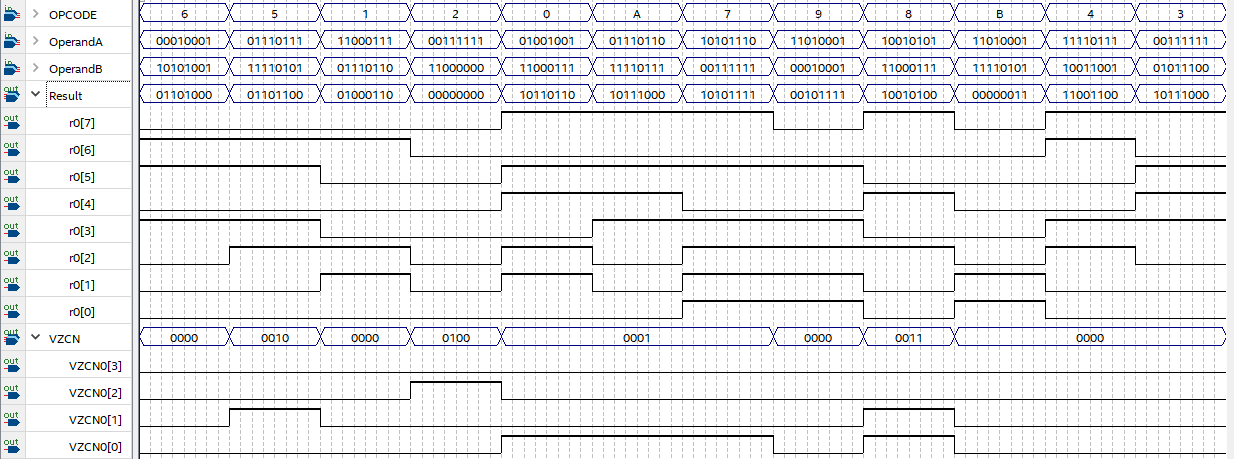
\includegraphics[width=\textwidth, height=\textheight, keepaspectratio=true]{valsimalu}
\caption{ALU Simulation Waveform}\label{alusim}
\end{figure}


\begin{figure}[ht]
\centering
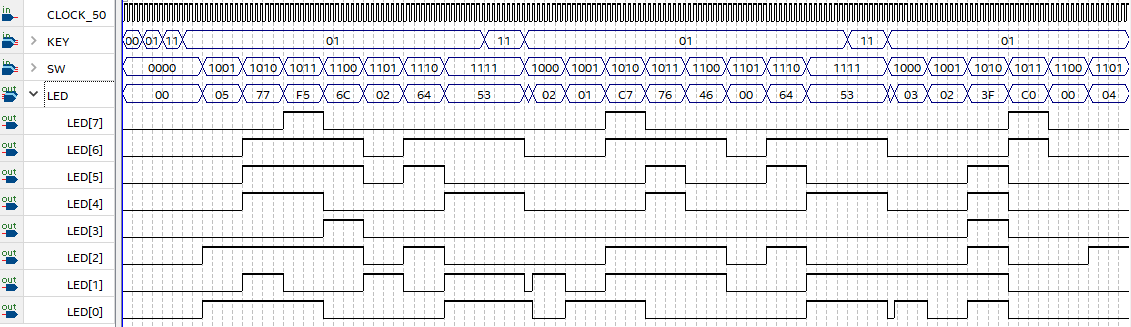
\includegraphics[width=\textwidth, height=\textheight, keepaspectratio=true]{valsim}
\caption{ALU Multiplexer Simulation Waveform}\label{alumuxsim}
\end{figure}
\clearpage

\section{Appendix B: Gate Count Calculations}
\label{gcount}
\begin{align*}
	HA&=XOR+AND=3AND+OR+NOT\\
	FA&=2HA+OR=6AND+3OR+2NOT\\
	RC8&=8FA=48AND+24OR+16NOT\\
	OP_{LSL}&=0\\
	OP_{ASR}&=0\\
	OP_{MULTI8}&=0\\
	OP_{NOT}&=8NOT\\
	OP_{AND}&=8AND\\
	OP_{XNOR}&=8XOR+8NOT=16AND+8OR+16NOT\\
	MUX_{1x2}&=NOT+2AND\\
	EQ_{4}&=4XNOR+3AND=11AND+4OR+8NOT\\
	EQ_{8}&=8XNOR+7AND=23AND+8OR+16NOT\\
	DEC_{4x2}&=4AND+2NOT\\
	MUX_{4x12}&=2DEC_{4x2Shared}+12AND\\
	MUX_{4x6}&=2DEC_{4x2Shared}+6AND\\
	MUX_{4x4}&=2DEC_{4x2Shared}+4AND\\
	MUX_{4x3}&=2DEC_{4x2Shared}+3AND\\
	MUX_{4x2}&=2DEC_{4x2Shared}+2AND\\
	OP_{ADD}&=OP_{SUB}=OP_{INC}=OP_{DEC}=OP_{NEG}\\
	&=8MUX_{4x2}+8MUX_{4x4}+8MUX_{4x3}+RC8\\
	&=2DEC_{4x2Shared}+120AND+24OR+16NOT\\
	OP_{MOD4}&=8MUX_{1x2}+OP_{NEG SHARED}\\
	ALU&=OP_{NOT}+OP_{AND}+OP_{XNOR}+8MUX_{4x12}+OP_{ADD}\\
	   &+OP_{MOD4}+2MUX_{4x6}+3EQ_{4}+3NOT+EQ_{8}+XOR\\
	   &=2DEC_{4x2}+OP_{NOT}+OP_{AND}+OP_{XNOR}\\
	   &+8MUX_{4x12}+2MUX_{4x6}+OP_{ADD}+2AND+OR+NOT\\
	   &+OP_{MOD4}+3EQ_{4}+3NOT+EQ_{8}\\
	   &=8AND+4NOT+8NOT+8AND+16AND+8OR+16NOT\\
	   &+96AND+12AND+120AND+24OR+16NOT\\
	   &+2AND+OR+NOT+8NOT+16AND+33AND\\
	   &+12OR+24NOT+23AND+8OR+16NOT\\
	   &=93NOT+334AND+53OR\\
	MYMUX&=2DEC_{4x2}+16AND=24AND+4NOT\\
	yourALUmux&=ALU+MYMUX=93NOT+334AND+53OR+24AND+4NOT\\
	&=97NOT+358AND+53OR
\end{align*}
\clearpage

\section{Appendix C: Propagation Delay Calculations}
\label{propdelay}
\begin{align*}
	t_{pdXNOR} &= 2t_{pdAND}+2t_{pdNOT} \\
	t_{pdEQ4} &= t_{pdXNOR}+2t_{pdAND} \\
			  &= 4t_{pdAND}+2t_{pdNOT}\\
	t_{pdHA} &= t_{pdXOR} = 2t_{pdAND}+t_{pdNOT} \\
	t_{pdFAs} &= 2t_{pdHA} = 4t_{pdAND}+2t_{pdNOT}  \\
	t_{pdFAc} &= 2t_{pdHA} + t_{pdOR} = 4t_{pdAND}+2t_{pdNOT} + t_{pdOR}  \\
	t_{pdRC8s} &= 7t_{pdFAc}+t_{pdFAs} = 32t_{pdAND}+16t_{pdNOT}+7t_{pdOR} \\
	t_{pdRC8c} &= 8t_{pdFAc} = 32t_{pdAND}+16t_{pdNOT} +8 t_{pdOR} \\
	t_{pdDEC} &= t_{pdNOT}+t_{pdAND} \\
	t_{pdmux4xA} &= t_{pdDEC}+t_{pdAND} = t_{pdNOT}+2t_{pdAND}\\
	t_{pdOverflow} &= 2t_{pdmux4xA}+ t_{pdRC8c}+t_{pdXOR}\\
			     &= 38t_{pdAND}+19t_{pdNOT} +8t_{pdOR}\\
	t_{pdALU} &= t_{pdOverflow} = 38t_{pdAND}+19t_{pdNOT} +8t_{pdOR}\\
	t_{pdMYMUX} &= t_{pdDEC} + t{pdAND} \\
	&= t_{pdNOT}+2t_{pdAND}\\
	t_{pdyourALUmux}&=t_{pdALU}+t_{pdMYMUX} \\
				&=40t_{pdAND}+20t_{pdNOT} +8t_{pdOR} 
\end{align*}
\clearpage


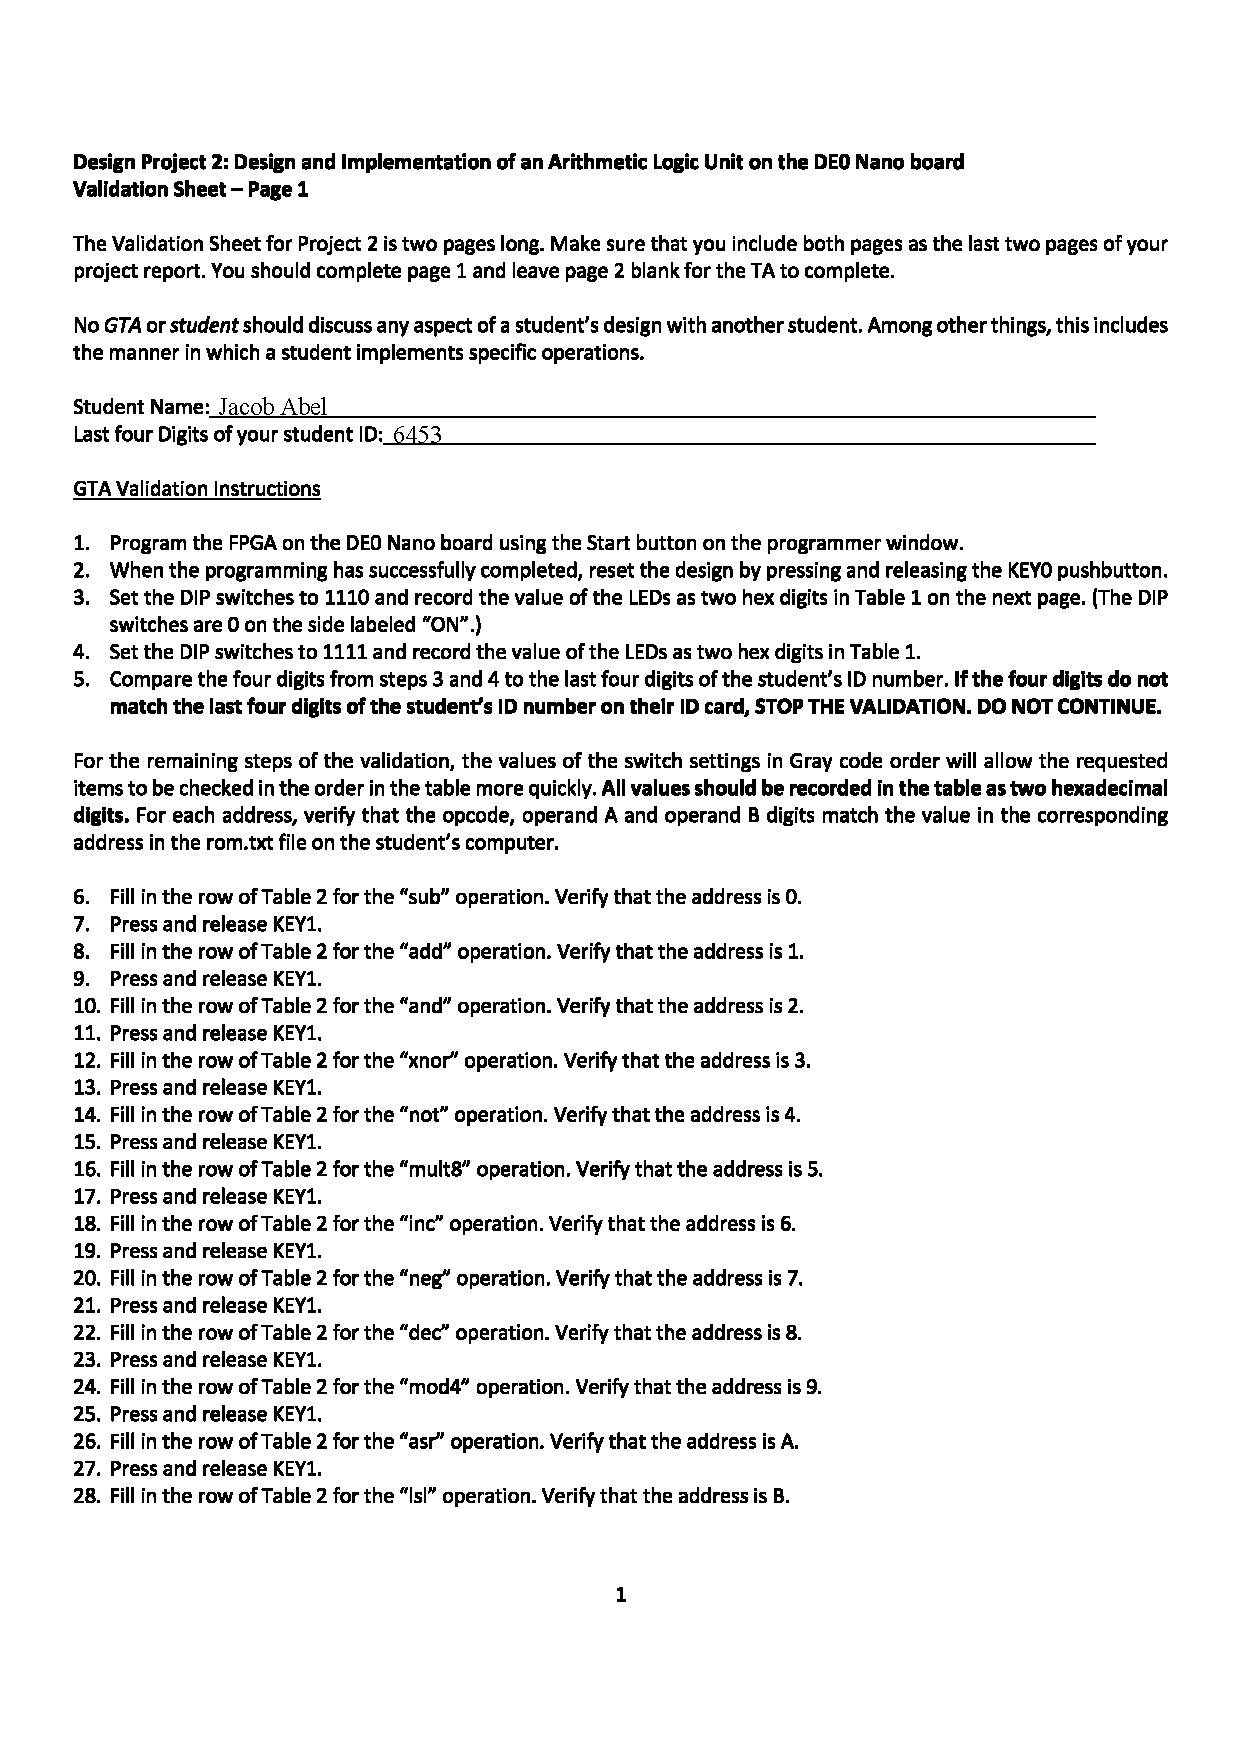
\includepdf[pages=-, noautoscale]{ValSheet.pdf}
\end{raggedright}
\end{document}
